Before doing the system configuration it is necessary to first setup all of the used tools, as will be next presented.

%**********************************************************
\subsection{Git}
In order to make collaboration easier, allowing change by multiple people to all be merged into one source, Git will be used. Git is the most commonly used version control system. Before using it, it is necessary to do the correct setup as shown bellow.
\begin{lstlisting}
$ sudo apt install git
$ git config --global user.name "John Doe"
$ git config --global user.email johndoe@example.com
$ git config --global core.editor subl
$ cd ~
$ git clone git@github.com:ESRGgroup9/slipad.git
\end{lstlisting}

With this steps, Git is installed in a local machine, username and user email is defined alongside with the default core editor. After this, one can clone the repository for this project, created in GitHub, by executing line 6.

%**********************************************************
\subsection{Buildroot}
Buildroot is a simple, efficient and easy-to-use tool used to generate this project's embedded Linux system, through cross-compilation. The steps in order to install Buildroot in a local machine is shown bellow.

\begin{lstlisting}
$ cd ~
$ mkdir buildroot
$ cd buildroot
$ wget https://buildroot.org/downloads/buildroot-2021.02.5.tar.gz
$ tar xzf buildroot-2021.02.5.tar.gz
$ cd buildroot-2021.02.5
\end{lstlisting}

After the installation is done, one can do the base configurations, essential to the support the rest of the configurations.
\begin{lstlisting}
$ make raspberrypi4_defconfig
$ make menuconfig
$ make xconfig
$ make 
$ make clean
\end{lstlisting}

The first command is used to configure a kernel image for the Raspberry Pi 4, as it does the necessary configurations regarding hardware handling along with fetching some board specific packages. Then with the second and third commands, one can generate the graphic interface seen in figure \ref{fig:menuconfig}, presenting several sub-menus. 

\begin{figure}[H]
	\centering	
	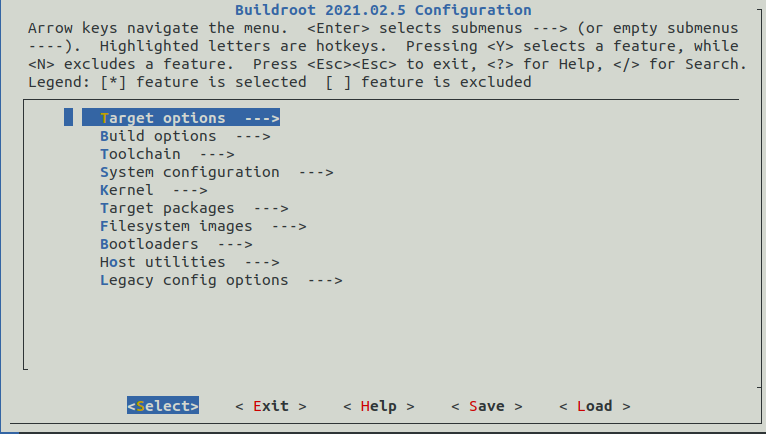
\includegraphics[width=.74\textwidth]{11configs/menuconfig}
	\caption{Buildroot menuconfig.}
	\label{fig:menuconfig}
\end{figure}

%**********************************************************
\subsection{OpenCV}

\begin{lstlisting}
$ cd ~/buildroot/buildroot-2021.02.5/output/build/opencv3-3.4.13/buildroot-build
$ cmake-gui
$ cmake .
$ make -j8
$ sudo make install
\end{lstlisting}

%**********************************************************
\subsection{Qt Creator}

The Qt Creator IDE was used to create an application that is used by the operator to interact with the system. The IDE instalation is done by downloading the open-source online installer present on the official site, in the download page \cite{qt_creator}. In the figure \ref{fig:qt_instalation} is shown all the packages installed for this IDE.

\begin{figure}[H]
	\centering	
	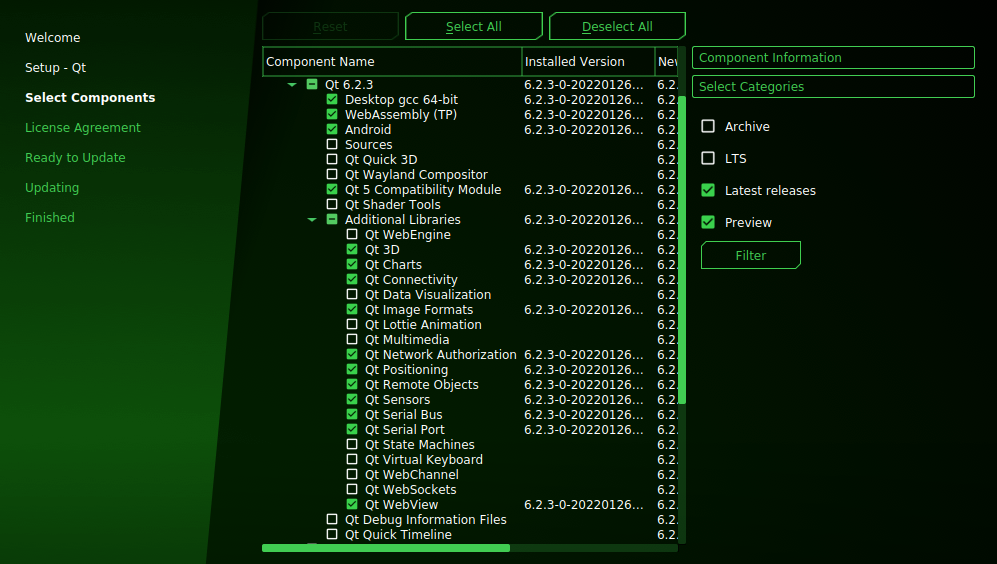
\includegraphics[width=.80\textwidth]{11configs/qt_instalation}
	\caption{Qt Creator: Instalation.}
	\label{fig:qt_instalation}
\end{figure}

Since one is deploying the application to an Android device, it was necessary to install and configure the Android Studio and SDK tools \cite{android_studio}, and also Android NDK \cite{android_ndk} in the Qt Creator. To install the Android Studio run \verb|<path-to-android-studio>/android-studio/bin/studio.sh|. Next, one needs to configure the platform of the Android Studio accordingly to the android phone version. The Android NDK must be the \verb|r23| version, and the Qt creator configure the packages missing.

It is also necessary to install a Java SE Development (JDK) \cite{java}. The JDK version shouldn't be the latest and the installed one was the version 11. Now, run \verb|<path-to-android-studio>/android/tools/bin/sdkmanager --licenses| in order to accept the licenses. 

At last, the \verb|QT -> Tools -> Options -> Devices -> Android|, sould look like shown in figure \ref{fig:qt_config}.

\begin{figure}[H]
	\centering	
	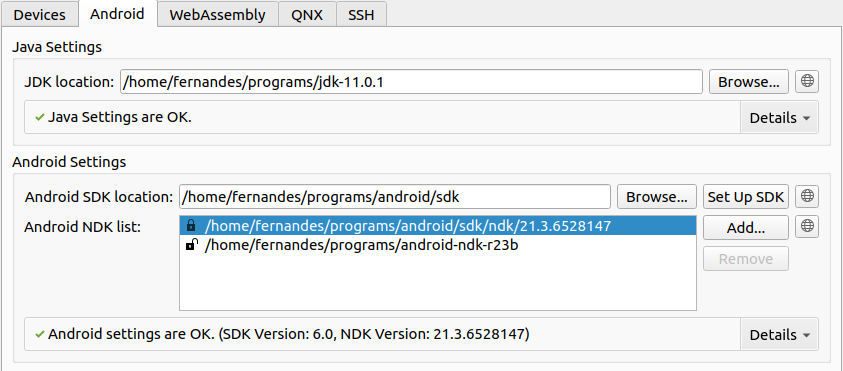
\includegraphics[width=.80\textwidth]{11configs/qt_config}
	\caption{Qt Creator: Configuration.}
	\label{fig:qt_config}
\end{figure}

%**********************************************************
\subsection{MySQL}
In order to have a fully managed database service to deploy cloud-native applications as MySQL, one has to firstly install it properly, as shown bellow.

\begin{lstlisting}
$ sudo apt-get install libmysqlclient-dev
\end{lstlisting}

First time runnning \verb|mysql|, one can create a strong password for \verb|mysql| access. After that, one can login into \verb|mysql| by typing:

\begin{lstlisting}
$ mysql -u root -p
\end{lstlisting}

%**********************************************************
\subsection{PHP}
In order to fetch data from the remote server database to the website that will present available parking spots, one uses PHP, which must first be configured. The following commands must be executed so that one gets a PHP client and PHP with MySql.

\begin{lstlisting}
$ sudo apt install php7.4-cli
$ sudo apt install php-mysqli
\end{lstlisting}

Knowing that fetching data from a remote database envolves secret keys, such as servername, username, port number, database password, it is usefull to have a \verb|.env| file which will contain all of them. In order to load those variables into the website index file one needs to setup \verb|phpdotenv| following the steps bellow. \cite{phpdotenv}

\begin{lstlisting}
$ sudo apt install composer
$ composer install
$ composer require vlucas/phpdotenv
\end{lstlisting}

%**********************************************************
\subsection{Google Maps Credentials}
In order for the website to present the parking spaces at a given location in a map, one uses Google Maps API. In order to generate a Google API key, one needs to go to Google API Console \cite{googleapi} and:

\begin{enumerate}
	\item Create a \textbf{new project};
	\item In API Manager go into \textbf{Library} and select \textbf{Google Maps Javascript API};
	\item Select the created project to enable APIs;
	\item Enable API;
	\item In API Manager go into \textbf{Credentials} and in \textbf{Create Credentials} click \textbf{Create API key}	
\end{enumerate}

After this steps, one may retrieve the generated key and use it within website source file. Make sure that this does not leak since it is a secret key that it is not meant be shared.